\documentclass[11pt,a4paper]{article}
\usepackage{amsmath, amssymb, amsthm}
\usepackage{geometry}
\usepackage{graphicx}
\usepackage{url}
\usepackage{hyperref}
\usepackage[dvipsnames]{xcolor}
\usepackage{mylistings}
\usepackage[font=small,skip=4pt]{caption}
\usepackage{chngcntr,tocloft}
\usepackage{fancyhdr}

\fancypagestyle{firstpage}{% define a custom header
  \fancyhf{}
  \renewcommand{\headrulewidth}{0pt}
  \fancyhead[L]{\footnotesize{Kaggle Notebook: \url{https://www.kaggle.com/code/muhammadumer2002/multivariate-ml}}
}}

\counterwithin*{figure}{section}
\counterwithin*{figure}{subsection}
\counterwithin*{figure}{subsubsection}

\addtolength{\cftfignumwidth}{2em}


\renewcommand{\thefigure}{%
\ifnum\value{subsection}=0
\thesection.\arabic{figure}%
\else
\ifnum\value{subsubsection}=0
\thesubsection.\arabic{figure}%
\else
\thesubsubsection.\arabic{figure}%
\fi
\fi
}

\renewcommand{\lstlistingname}{Algorithm}

\definecolor{codegreen}{rgb}{0,0.6,0}
\definecolor{codegray}{rgb}{0.5,0.5,0.5}
\definecolor{codepurple}{rgb}{0.58,0,0.82}
\definecolor{backcolour}{rgb}{0.9725,0.9725,0.9725}

\lstdefinestyle{mystyle}{
backgroundcolor=\color{backcolour},   
commentstyle=\color{codegreen},
keywordstyle=\color{magenta},
% numberstyle=\tiny\color{codegray},
stringstyle=\color{codepurple},
basicstyle=\ttfamily\footnotesize,
breakatwhitespace=false,         
breaklines=true,                 
captionpos=b,                    
keepspaces=true,                 
% numbers=left,                    
% numbersep=5pt,                  
showspaces=false,                
showstringspaces=false,
showtabs=false,                  
tabsize=2,
frame=tb,
framexleftmargin=2mm,
xleftmargin=2mm,
framexrightmargin=2mm,
xrightmargin=2mm,
% rulecolor=\color{black},
upquote=true,
aboveskip=3mm,
belowskip=3mm,
captionpos=b
}

\lstset{style=mystyle}

\parindent 0pt

\geometry{
  top=1in,
  bottom=1in,
  left=0.8in,
  right=0.8in
}
\renewcommand{\contentsname}{Contents}

\renewcommand{\baselinestretch}{1.25}
\renewcommand{\contentsname}{Contents}

\usepackage{hyperref}
\hypersetup{
colorlinks,
citecolor=blue,
filecolor=blue,
linkcolor=blue,
urlcolor=blue
}

\usepackage{enumitem}

\usepackage{cleveref}
\crefname{section}{\S}{\S\S}
\Crefname{section}{\S}{\S\S}
\crefname{subsection}{\S}{\S\S}
\Crefname{subsection}{\S}{\S\S}

\begin{document}

% Titlepage
\newpage
\begin{titlepage}
  \vspace*{\fill} % add vertical space before content
  \centering
  \huge{\textbf{CS470 -- Machine Learning}} \\
  \huge{Assignment 1} \\ 
  \LARGE{
    \href{
      https://www.kaggle.com/code/muhammadumer2002/multivariate-ml}{Kaggle Notebook Link}} \\ [0.75cm]
  \begin{figure}[ht!]
    \centering
    
\includegraphics[width=0.5\textwidth]{figs/nust.pdf}
  \end{figure}
  \vspace {0.75cm}
  \Large{By} \\
  \Large{\textbf{Muhammad Umer}\quad(CMS -- 345834)} \\
  \Large{\textbf{Danial Ahmad}\quad(CMS -- 331388)} \\[0.75cm]
  \Large{Instructor} \\
  \Large{\textbf{Dr. Ahmad Salman}} \\[0.75cm]
  \Large{School of Electrical Engineering and Computer Science (SEECS) \\
    National University of Sciences and Technology (NUST) \\
    Islamabad, Pakistan} \\ [0.75 cm]
  \Large{\today}
  \vspace*{\fill} % add vertical space after content
\end{titlepage}

% \tableofcontents
% \newpage

\setcounter{page}{1}
\thispagestyle{firstpage}

\section{Task 1 -- Multivariate Gaussian Classifier}
Using Fisher's Iris multivariate data (in .mat file), perform multivariate Gaussian classification. This a 4D data with three classes and corresponding labels.

\hrulefill

\textbf{Solution}
Before proceeding, we import relevant libraries, load the data, and define some parameters.

\begin{lstlisting}[language=Python]
# Importing libraries
import numpy as np
import matplotlib.pyplot as plt
from scipy.io import loadmat
from sklearn import metrics
from IPython.lib.pretty import pretty
import pandas as pd

# Plotting settings: STIX fonts
plt.rcParams["font.family"] = "STIXGeneral"

# Loading data
data = loadmat("iris_data.mat")["iris"]  # 150x5
features = data[:, :-1]  # 150x4
labels = data[:, -1]  # 150x1
split_val = 100  # 100 for training, len(data) - 100 for testing

# Class labels
# Ref: https://en.wikipedia.org/wiki/Iris_flower_data_set
class_names = ["Setosa", "Versicolor", "Virginica"]
class_ids = np.unique(labels).astype(int)  # 0, 1, 2

print("Data shape:", data.shape)
print("Features shape:", features.shape)
print("Labels shape:", labels.shape)
print("Class labels:", class_names)
print("Class IDs:", class_ids)
\end{lstlisting}

% Output listing
\begin{lstlisting}[numbers=none, framexleftmargin=2mm, xleftmargin=2mm, framexrightmargin=2mm, xrightmargin=2mm]
# Output information
>>> Data shape:      (150, 5)
>>> Features shape:  (150, 4)
>>> Labels shape:    (150, 1)
>>> Class labels:    ['Setosa', 'Versicolor', 'Virginica']
>>> Class IDs:       [0 1 2]
\end{lstlisting}

\hrulefill

Perform the following tasks:

\begin{enumerate}[leftmargin=*]
\item Randomly shuffle the data and corresponding labels.

\begin{lstlisting}[language=Python]
m = len(data)  # Number of samples
indices = np.random.permutation(m)  # Create a list of shuffled indices from 0 to m-1
X = features[indices]  # Shuffle the dataset
y = labels[indices]  # Shuffle the labels
\end{lstlisting}

\fancyhf{} % sets both header and footer to nothing

\item Use first 100 samples (rows) in training dataset.

\begin{lstlisting}[language=Python]
# Split the dataset into training and test datasets
X_train = X[: split_val]
y_train = y[: split_val]

print("X_train shape:", X_train.shape)
print("y_train shape:", y_train.shape)
\end{lstlisting}

% Output listing
\begin{lstlisting}[numbers=none, framexleftmargin=2mm, xleftmargin=2mm, framexrightmargin=2mm, xrightmargin=2mm]
# Output information
>>> X_train shape: (100, 4)
>>> y_train shape: (100,)
\end{lstlisting}

  \item Use remaining 50 samples in test dataset.

\begin{lstlisting}[language=Python]
X_test = X[split_val :]
y_test = y[split_val :]

print("X_test shape:", X_test.shape)
print("y_test shape:", y_test.shape)
\end{lstlisting}

% Output listing
\begin{lstlisting}[numbers=none, framexleftmargin=2mm, xleftmargin=2mm, framexrightmargin=2mm, xrightmargin=2mm]
# Output information
>>> X_test shape: (50, 4)
>>> y_test shape: (50,)
\end{lstlisting}

\item Scatter plot first two dimensions of each class.

\begin{lstlisting}[language=Python]
plt.figure(figsize=(7, 5))
for i in class_ids:
    plt.scatter(
        X_train[y_train == i, 0],
        X_train[y_train == i, 1],
        label=class_names[i - 1],
        alpha=0.7,
    )
plt.xlabel("Feature 1")
plt.ylabel("Feature 2")
plt.legend()
plt.show()
\end{lstlisting}

\begin{figure}[ht!]
  \centering
  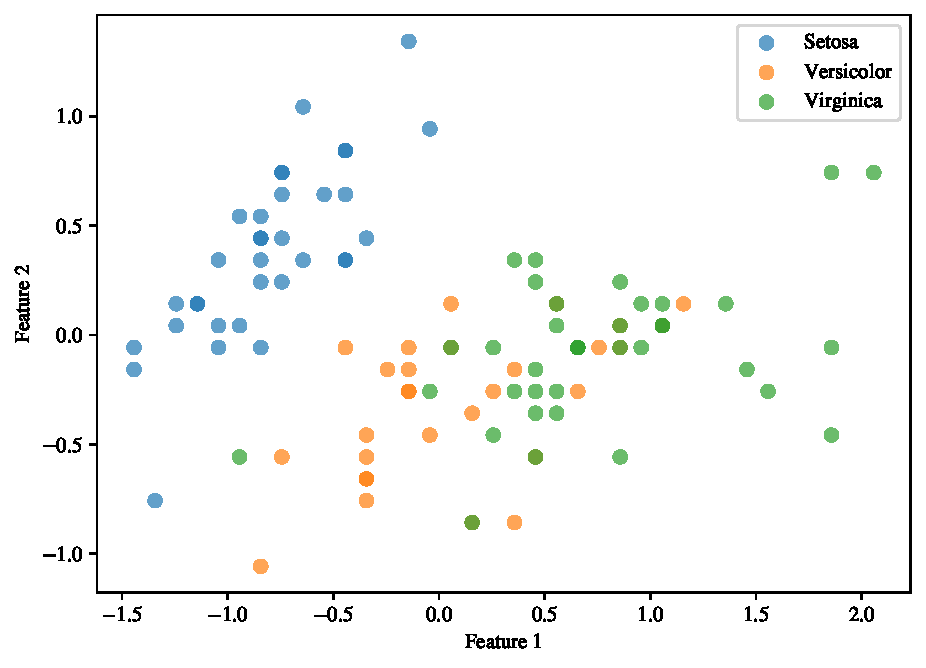
\includegraphics[width=0.55\textwidth]{figs/scatter_plot.pdf}
  \caption{Scatter plot of the first two dimensions.}
\end{figure}

\item Using Gaussian discriminant function without dropping any term, perform classification and show the result in a form of a confusion matrix.

The Gaussian discriminant function is given by
\[g_i(\mathbf{x}) = -\frac{1}{2}(\mathbf{x}-\mathbf{m}_i)^T\mathbf{S}_i^{-1}(\mathbf{x}-\mathbf{m}_i) - \frac{1}{2}\ln|\mathbf{S}_i| + \ln \hat{P}(C_i),\]

where $\mathbf{m}_i$ and $\mathbf{S}_i$ are the estimates of the mean and covariance matrix of the data in each class $C_i$.

\begin{lstlisting}[language=Python]
# Estimating parameters
priors = dict()
means = dict()
covs = dict()

for i in class_ids:
    priors[i] = np.sum(y_train == i) / len(y_train)
    means[i] = np.mean(X_train[y_train == i], axis=0)  # each mean vector is 1x4
    covs[i] = np.cov(X_train[y_train == i].T)  # each cov mat is 4x4
    
print("Priors:\n", pretty(priors))
print("\nMeans:\n", pretty(means))
print("\nCovariances:\n", pretty(covs))

def discriminant_function(x, i):
    """Gaussian discriminant function"""
    return (
        -0.5 * np.log(np.linalg.det(covs[i]))
        - 0.5 * (x - means[i]).T @ np.linalg.inv(covs[i]) @ (x - means[i])
        + np.log(priors[i])
    )  # @ is matrix multiplication (dot product)

y_pred = np.zeros(len(y_test))

for i in range(len(y_test)):
    x = X_test[i]
    g = np.zeros(len(class_ids))
    for j in class_ids:
        g[j - 1] = discriminant_function(x, j)
    y_pred[i] = np.argmax(g) + 1  # +1 because class_ids start from 1

print("y_pred:\n", y_pred)
print("\ny_test:\n", y_test)

# Confusion matrix
cm = metrics.confusion_matrix(y_test, y_pred)
cm_display = metrics.ConfusionMatrixDisplay(cm, display_labels=class_names)
cm_display.plot(cmap=plt.cm.Blues)
plt.show()
\end{lstlisting}

% Output listing
\begin{lstlisting}[numbers=none, framexleftmargin=2mm, xleftmargin=2mm, framexrightmargin=2mm, xrightmargin=2mm]
# Output information
>>> Priors:
{1: 0.33, 2: 0.32, 3: 0.35}

>>> Means:
{1: array([-0.82515152,  0.39721212, -2.27315152, -0.94478788]),
2: array([ 0.09416667, -0.31670833,  0.513875  ,  0.12879167]),
3: array([ 0.68809524, -0.09447619,  1.77628571,  0.77209524])}

>>> Covariances:
{1: array([[0.09153409, 0.09835227, 0.00778409, 0.01178977],
  [0.09835227, 0.16880682, 0.00897727, 0.00911932],
  [0.00778409, 0.00897727, 0.01945076, 0.00397727],
  [0.01178977, 0.00911932, 0.00397727, 0.01443182]]),
2: array([[0.29532258, 0.09004032, 0.18657258, 0.05923387],
  [0.09004032, 0.09539315, 0.06763105, 0.03172379],
  [0.18657258, 0.06763105, 0.21111895, 0.07017137],
  [0.05923387, 0.03172379, 0.07017137, 0.03434476]]),
3: array([[0.38339496, 0.09737815, 0.29653782, 0.0397479 ],
  [0.09737815, 0.11652101, 0.08454622, 0.0644958 ],
  [0.29653782, 0.08454622, 0.29231933, 0.05571429],
  [0.0397479 , 0.0644958 , 0.05571429, 0.08621849]])}
  \end{lstlisting}

\begin{figure}[ht!]
  \centering
  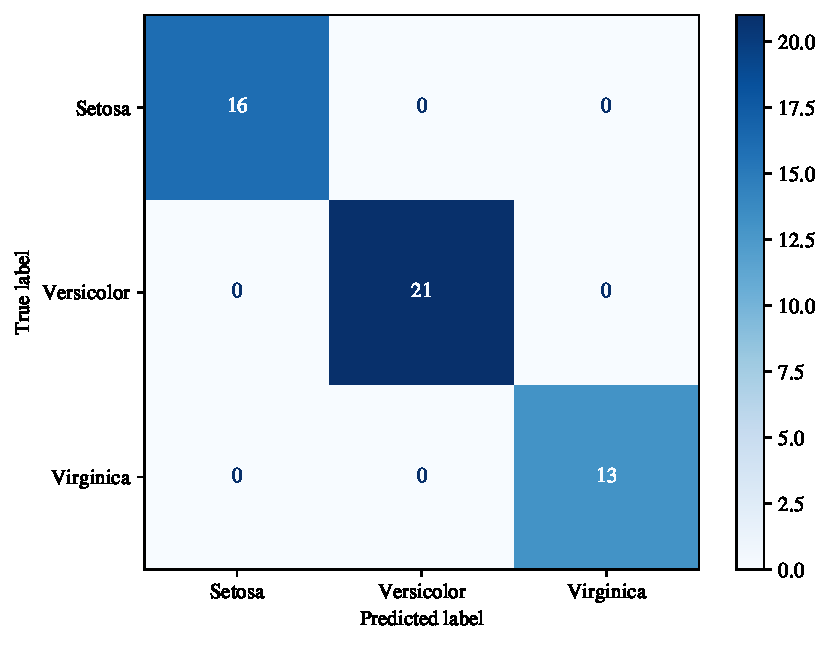
\includegraphics[width=0.55\textwidth]{figs/confusion_matrix.pdf}
  \caption{Confusion matrix of the Gaussian discriminant function.}
\end{figure}

\item Can you drop any term in the discriminant function? Why?

Yes, we can drop the prior probability term in the discriminant function. This is because the prior probability is the nearly the same for all the classes, i.e., Fisher's Iris is a balanced dataset. Hence, the prior probability term will not affect the classification results.

\begin{lstlisting}[language=Python]
def modified_discriminant_function(x, i): # Modified for equal priors
    return -0.5 * np.log(np.linalg.det(covs[i])) - 0.5 * (
        x - means[i]
    ).T @ np.linalg.inv(covs[i]) @ (x - means[i])

y_pred = np.zeros(len(y_test))

for i in range(len(y_test)):
    x = X_test[i]
    g = np.zeros(len(class_ids))
    for j in class_ids:
        g[j - 1] = discriminant_function(x, j)
    y_pred[i] = np.argmax(g) + 1  # +1 because class_ids start from 1

print("y_pred:\n", y_pred)
print("\ny_test:\n", y_test)

cm = metrics.confusion_matrix(y_test, y_pred)
cm_display = metrics.ConfusionMatrixDisplay(cm, display_labels=class_names)
cm_display.plot(cmap=plt.cm.Blues)
plt.show()
\end{lstlisting}

        \begin{figure}[ht!]
          \centering
          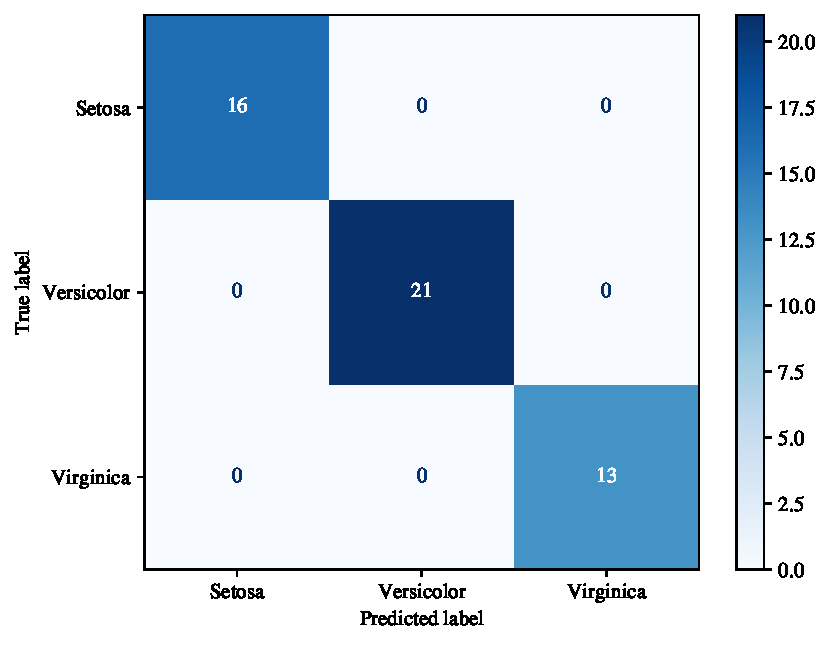
\includegraphics[width=0.55\textwidth]{figs/mod_confusion_matrix.pdf}
          \caption{Confusion matrix of the modified Gaussian discriminant function.}
        \end{figure}

\end{enumerate}

\newpage

\section{Task 2 -- Multivariate Linear Regression}
Using US CDC data of weekly flu estimates over a year, perform multivariate
regression (in Matlab \textbf{load flu}). This data comprises weekly flu estimates of nine US regions (column-2 to 10). Column-1 is the date and last column (WtdILI) is the CDC's national estimate, take this as label \textbf{r}. Since there are nine regions against each date, this is $d=9$ dimensional data.

Visualize data as:

\begin{lstlisting}[language=Python]
load flu
Y = double(flu(:,2:end-1));
[n,d] = size(Y);
x = flu.WtdILI;
figure;
regions = flu.Properties.VarNames(2:end-1);
plot(x,Y,'x')
legend(regions,'Location','NorthWest')
\end{lstlisting}

\begin{figure}[ht!]
  \centering
  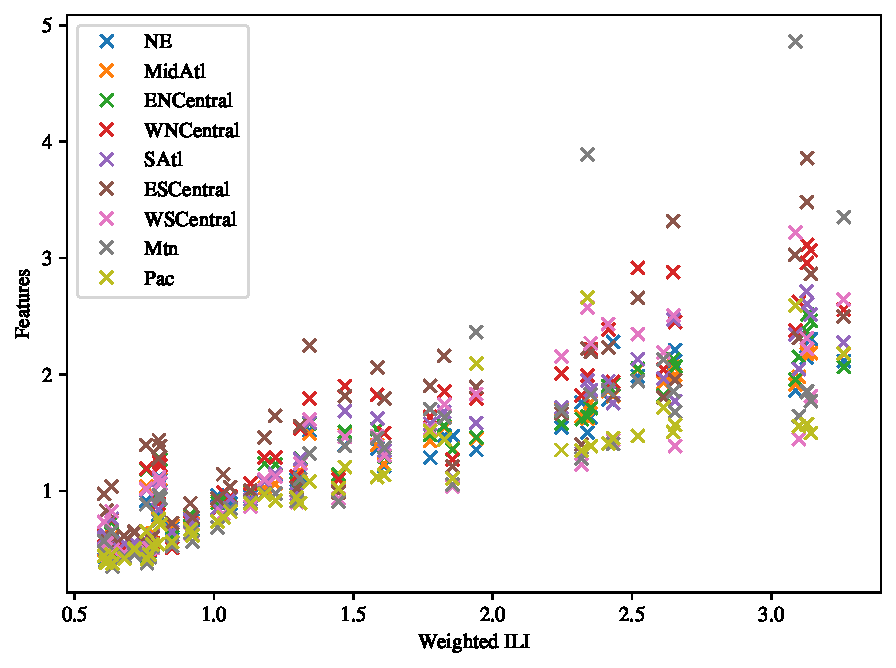
\includegraphics[width=0.65\textwidth]{figs/flu_data.pdf}
  \caption{Visualizing the US CDC flu data.}
\end{figure}

\hrulefill

\textbf{Solution}
Before proceeding, we convert the US CDC dataset to a .mat and a .csv file.

\begin{lstlisting}[language=Matlab]
% Export files
savemat = [x Y];
save("flu_data.mat", "savemat")
t = dataset2table(flu);
writetable(t, "flu_data.csv")
\end{lstlisting}

\hrulefill

Perform the following tasks:

\enumerate[leftmargin=*]
\item Save .mat file for flu from Matlab to work in Python.

The following MATLAB code can be used to save the .mat file for UC CDC Flu Data from MATLAB to work in Python.

\begin{lstlisting}[language=Matlab]
savemat = [x Y];  % concatenate x and Y
save("flu_data.mat", "savemat")
\end{lstlisting}

where \lstinline{x} and \lstinline{Y} are the variables in MATLAB workspace as per the manual.

\begin{lstlisting}[language=Python]
# Multivariate linear regression
data = loadmat("flu_data.mat")["savemat"]
X = data[:, 1:]  # 52x9
r = data[:, 0]  # 52x1

print("X shape:", X.shape)
print("r shape:", r.shape)
\end{lstlisting}

% Output listing
\begin{lstlisting}[numbers=none, framexleftmargin=2mm, xleftmargin=2mm, framexrightmargin=2mm, xrightmargin=2mm]
# Output information
>>> X shape: (52, 9)
>>> r shape: (52,)
\end{lstlisting}

\item Find the parameters $w_j$, $j = 1, 2, \ldots, 9$ for the estimator
\[g(x \mid w) = w_0 + w_1 x_1^t + w_2 x_2^t + \cdots + w_d x_d^t.\]

To find the parameters $w_j$, $j = 1, 2, \ldots, 9$ for the estimator, we need to minimize the sum of squared errors (SSE) between the estimated values and the actual values. For that, we need to write our matrices as:

$$\mathbf{X} = \begin{bmatrix} 1 & x_{11} & x_{12} & \cdots & x_{1d} \\ 1 & x_{21} & x_{22} & \cdots & x_{2d} \\ \vdots & \vdots & \vdots & \ddots & \vdots \\ 1 & x_{N1} & x_{N2} & \cdots & x_{Nd} \end{bmatrix}, \: \mathbf{w} = \begin{bmatrix} w_0 \\ w_1 \\ \vdots \\ w_d \end{bmatrix}, \: \mathbf{r} = \begin{bmatrix} r_1 \\ r_2 \\ \vdots \\ r_N \end{bmatrix}.$$

Note that we need to append a column of ones to the data matrix $\mathbf{X}$ to account for the bias term $w_0$.

After that, we can solve for the least squared solution using the following equation

$$\mathbf{w} = (\mathbf{X}^TX)^{-1}\mathbf{X}^T\mathbf{r}.$$

\begin{lstlisting}[language=Python]
# Append a column of ones to X
X_prime = np.hstack((np.ones((N, 1)), X))
print("X shape:", X_prime.shape)

# Estimating parameters
w = np.linalg.inv(X_prime.T @ X_prime) @ X_prime.T @ r  # Moore-Penrose pseudoinverse

print("\nw shape:", w.shape)
print("w:\n", w)
\end{lstlisting}

% % Output listing
% \begin{lstlisting}[numbers=none, framexleftmargin=2mm, xleftmargin=2mm, framexrightmargin=2mm, xrightmargin=2mm]
% # Output information
% >>> X shape: (52, 10)

% >>> w shape: (10,)
% >>> w:
% [-0.00485246  0.98435106  0.57276929 -1.43543044  0.49793484  0.9254393
%  -0.19997715 -0.37716256  0.2357128   0.05934519]
% \end{lstlisting}

\item Observe the structure of g(x|w) which should be [N x 1].

\begin{lstlisting}[language=Python]
# Observing the structure of g(x|w)
g = w[0] + X @ w[1:]  # Linear regression
g = g.reshape(-1, 1)  # 52x1

print("\ng(x|w) shape:", g.shape)
\end{lstlisting}

% Output listing
\begin{lstlisting}[numbers=none, framexleftmargin=2mm, xleftmargin=2mm, framexrightmargin=2mm, xrightmargin=2mm]
# Output information
>>> g(x|w) shape: (52, 1)
\end{lstlisting}


\item Plot both $g(x \mid w)$ and label vector $\mathbf{r}$ on the same figure to compare.

\begin{lstlisting}[language=Python]
# Plotting
plt.figure(figsize=(7, 5))
plt.plot(r, "x", color="red", markeredgewidth=1.5)
plt.plot(g, "-")
plt.plot(g, "o", color="black", markerfacecolor="none")
plt.legend(["Actual", "Predicted"])
plt.xlabel("Samples")
plt.ylabel("Weighted ILI")
plt.show()
\end{lstlisting}

\begin{figure}[ht!]
  \centering
  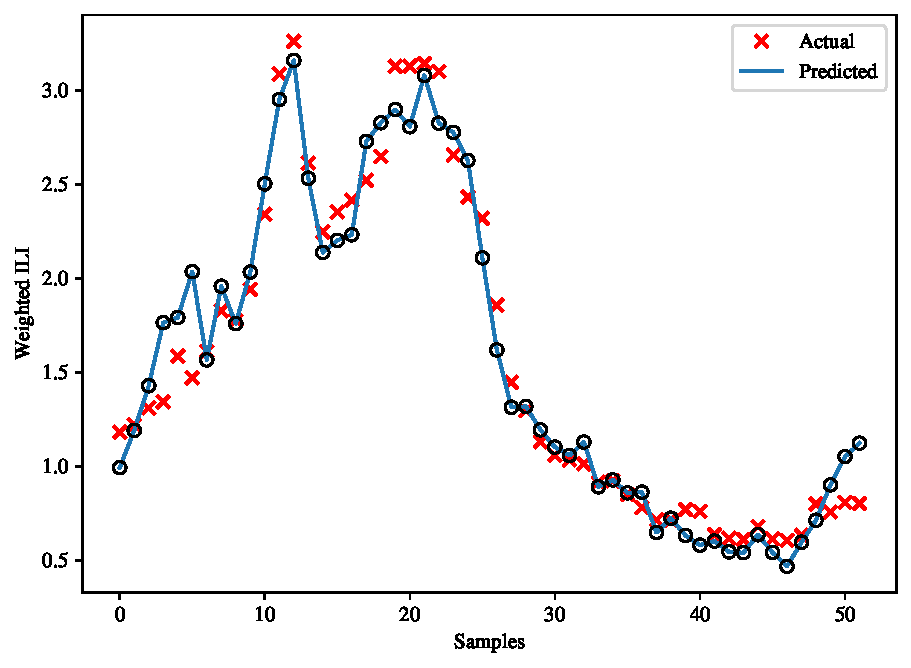
\includegraphics[width=0.65\textwidth]{figs/flu_data_pred.pdf}
  \caption{Linear regression of the weighted ILI.}
\end{figure}

\end{document}